\documentclass[12pt,compress,ngerman,utf8,t]{beamer}
\usepackage[ngerman]{babel}
\usepackage{calc}
\usepackage{ragged2e,wasysym,multicol,mathtools,tikz,txfonts,ifthen,wasysym,xspace}
\usepackage[all]{xy}
\usetikzlibrary{calc,shapes.callouts,shapes.arrows}
\usepackage[protrusion=true,expansion=true]{microtype}
\hypersetup{colorlinks=true}

\graphicspath{{images/}}

\title[A primer to the set-theoretic multiverse philosophy]{$\varheartsuit$ A
primer to the set-theoretic multiverse philosophy $\varheartsuit$}
\author[Ingo Blechschmidt]{\scriptsize\textcolor{white}{
\vspace*{-1em} \\
\textbf{36th Chaos Communication Congress} \\
\emph{Questions are very much welcome! Please interrupt me mid-sentence.} \\
\medskip
Ingo Blechschmidt \\
University of Augsburg}}

%\usetheme{Warsaw}
\useinnertheme[shadow=false]{rounded}
\useoutertheme{split}
\usecolortheme{orchid}
\usecolortheme{whale}
\setbeamerfont{block title}{size={}}

\useinnertheme{rectangles}

\usecolortheme{seahorse}
\definecolor{mypurple}{RGB}{150,0,255}
\setbeamercolor{structure}{fg=mypurple}
\definecolor{myred}{RGB}{150,0,0}
\definecolor{darkred}{RGB}{240,0,0}
\setbeamercolor*{title}{bg=myred,fg=white}
\setbeamercolor*{titlelike}{bg=myred,fg=white}
\definecolor{darkdarkred}{RGB}{180,0,0}
\definecolor{gold}{RGB}{255,115,0}

\newenvironment<>{hilblock}{
  \begin{minipage}{\textwidth}
    \begin{actionenv}#1
      \def\insertblocktitle{}
      \par
      \usebeamertemplate{block begin}}{
      \par
      \usebeamertemplate{block end}
    \end{actionenv}
  \end{minipage}}

\usefonttheme{serif}
\usepackage[T1]{fontenc}
\usepackage{libertine}

\renewcommand{\_}{\mathpunct{.}\,}
\renewcommand{\P}{\text{P}}
\newcommand{\aaa}{\mathfrak{a}}
\newcommand{\bbb}{\mathfrak{b}}
\newcommand{\ccc}{\mathfrak{c}}
\newcommand{\mmm}{\mathfrak{m}}
\newcommand{\ppp}{\mathfrak{p}}
\newcommand{\ZFC}{\textsc{zfc}\xspace}
\newcommand{\CH}{\textsc{ch}\xspace}
\newcommand{\NP}{\text{NP}}
\newcommand{\NPC}{\text{NP{-}C}}
\newcommand{\PSPACE}{\text{PSPACE}}
\newcommand{\PSPACEC}{\text{PSPACE{-}C}}
\newcommand{\EXP}{\text{EXP}}
\newcommand{\BB}{\mathbb{B}}
\newcommand{\M}{\mathcal{M}}
\newcommand{\R}{\mathrm{R}}
\newcommand{\NN}{\mathbb{N}}
\newcommand{\RR}{\mathbb{R}}
\newcommand{\Eff}{\mathrm{Eff}}
\newcommand{\TM}{\mathrm{TM}}
\newcommand{\STM}{\mathrm{STM}}
\newcommand{\RW}{\mathrm{RW}}
\newcommand{\lambdaC}{\lambda\mathrm{C}}
\newcommand{\PA}{\mathrm{PA}}
\newcommand{\goedel}[1]{\ulcorner #1 \urcorner}
\newcommand{\Prov}{\mathrm{Prov}}
\newcommand{\True}{\mathrm{True}}
\newcommand{\Con}{\mathrm{Con}}
\newcommand{\proves}{\vdash}
\newcommand{\defeq}{\vcentcolon=}

\newcommand{\pointthis}[4]{%
  \tikz[remember picture,baseline]{\node[anchor=base,inner sep=0,outer sep=0]%
    (#3) {#3};\node[overlay,rectangle callout,%
      callout relative pointer={(#1)},fill=blue!20] at
        ($(#3.north)+(#2)$) {#4};}}

\newcommand{\kasten}[1]{%
  \setlength{\fboxrule}{2pt}%
  \setlength{\fboxsep}{8pt}%
  {\usebeamercolor[fg]{item}\fbox{\usebeamercolor[fg]{normal text}\parbox{0.2cm}{#1}}}}%

\newcommand{\slogan}[1]{%
  \begin{center}%
    \setlength{\fboxrule}{2pt}%
    \setlength{\fboxsep}{8pt}%
    {\usebeamercolor[fg]{item}\fbox{\usebeamercolor[fg]{normal text}\parbox{0.88\textwidth}{#1}}}%
  \end{center}%
}

\newcommand{\code}[1]{%
  \begin{center}%
    \setlength{\fboxrule}{1pt}%
    \setlength{\fboxsep}{8pt}%
    {\fbox{\parbox{0.81\textwidth}{#1}}}%
  \end{center}%
}

\setbeamertemplate{navigation symbols}{}

\setbeamertemplate{title page}[default][colsep=-1bp,rounded=false,shadow=false]
\setbeamertemplate{frametitle}[default][colsep=-2bp,rounded=false,shadow=false,center]

\newcommand{\hil}[1]{{\usebeamercolor[fg]{item}{\textbf{#1}}}}
\newcommand{\bad}[1]{\textbf{\textcolor{darkred}{#1}}}
\setbeamertemplate{headline}{}
\setbeamertemplate{frametitle}{%
  \vskip1.2em%
  \leavevmode%
  \begin{beamercolorbox}[dp=1ex,center]{}%
      \usebeamercolor[fg]{item}{\textbf{\textsf{\Large \insertframetitle}}}
  \end{beamercolorbox}%
}

\setbeamertemplate{footline}{%
  \leavevmode%
  \hfill%
  \begin{beamercolorbox}[ht=2.25ex,dp=1ex,right]{}%
    \usebeamerfont{date in head/foot}
    \insertframenumber\,/\,\inserttotalframenumber\hspace*{1ex}
  \end{beamercolorbox}%
  \vskip0pt%
}

\newcommand{\backupstart}{
  \newcounter{framenumberpreappendix}
  \setcounter{framenumberpreappendix}{\value{framenumber}}
}
\newcommand{\backupend}{
  \addtocounter{framenumberpreappendix}{-\value{framenumber}}
  \addtocounter{framenumber}{\value{framenumberpreappendix}}
}

\newcommand{\portrait}[4]{\begin{column}{#3\textwidth}\centering\includegraphics[height=#4\textheight]{#1}\\{\scriptsize #2\par}\end{column}}

\setbeameroption{show notes}


\begin{document}

\addtocounter{framenumber}{-1}

{\usebackgroundtemplate{\begin{minipage}{\paperwidth}\vspace*{0.3cm}\centering\scriptsize\vspace*{3.95cm}\includegraphics[width=\paperwidth]{sun3}\end{minipage}}
\begin{frame}[c]
  \centering

  \bigskip
  \bigskip
  \bigskip
  \bigskip
  \Large

  \hil{A primer to the \\ \mbox{$\varheartsuit$ set-theoretic multiverse
  philosophy $\varheartsuit$}}

  \bigskip
  
  \footnotesize
  \textit{-- an invitation --}
  \bigskip
  \bigskip
  \medskip

  \textcolor{black}{
    \textbf{36th Chaos Communication Congress} \\
    \emph{Questions are very much welcome! Please interrupt me mid-sentence.}
  }
  \bigskip
  \bigskip

  \tiny
  \textcolor{white}{
    Ingo Blechschmidt \\
    University of Augsburg
  }

  \par
\end{frame}}

% \begin{document}

\begin{frame}{Prehistory}
  \centering
  \large
  \scalebox{3}{\frownie} \\
  \hil{Inconsistency} \\
  at the \textcolor{darkdarkred}{heart} of mathematics $\sim$ 1900 \\
  \small
  ``Let $R$ be the set of all those sets which don't contain themselves.''
  \par
  \normalsize
  \bigskip
  \bigskip
  \pause

  \scalebox{3}{\smiley} \\
  \hil{Formal proofs as the \textcolor{gold}{gold standard} \\ to judge correctness} $\sim$ 1920 \\
  \small
  Zermelo--Fraenkel set theory with the axiom of choice, \ZFC
  \par
  \normalsize
  \bigskip
  \bigskip
  \pause

  \scalebox{3}{\frownie} \\
  \hil{Incompleteness} $\sim$ 1931
\end{frame}

\begin{frame}{An outline of \ZFC}
  \hil{Axioms} of \ZFC include:
  \begin{enumerate}\small
    \item $\exists x\_ \forall y\_ \neg(y \in x)$ \\
    ``There is a set~$x$ such that for every set~$y$, it is not the case that~$y$ is
    an element of~$x$.''
    \item $\forall x\_ \forall y\_ \exists w\_ (x \in w \wedge y \in w)$ \\
    \mbox{``Given any sets $x$ and $y$, there is a set which contains $x$ and~$y$.''}
    \item $\forall x\_ \exists z\_ \forall w\_ ((\forall y\_ (y \in w
    \Rightarrow y \in x)) \Rightarrow w \in z)$. \\
    \mbox{``Given any set $x$, there is a set which contains all subsets of $x$.''}
  \end{enumerate}
  \bigskip

  \hil{Inference rules} of~\ZFC include:
  \begin{enumerate}\small
    \item From $\varphi \wedge \psi$ deduce $\varphi$.
    \item Modus ponens: From $\varphi$ and $\varphi\Rightarrow\psi$ deduce $\psi$.
    \item Law of excluded middle: Deduce $\varphi \vee \neg\varphi$.
  \end{enumerate}
  \bigskip

  \textbf{Def.} ``$\ZFC \vdash \varphi$'' means: There is a~\ZFC-proof
  of~$\varphi$.

  \textbf{Ex.} $\ZFC \vdash 2+2=4$,
  $\ZFC \not\vdash 2+2=5$.
\end{frame}

\begin{frame}{Foundational incompleteness}
  \justifying
  \textbf{Def.} A formal system~$S$ (such as~\ZFC) is \hil{inconsistent} if and
  only if it proves a contradiction: $S \vdash 1 = 0$.
  \pause

  \begin{hilblock}\justifying
    \textbf{Gödel's first incompleteness theorem.}
    Let~$S$ be a ``reasonable'' formal system (such as~$\ZFC$).
    Then there are mathematical statements~$\varphi$ such that, if there is
    an~$S$-proof of~$\varphi$ or if there is an~$S$-proof of~$\neg\varphi$ (the
    negation of~$\varphi$), then~$S$ is inconsistent.
  \end{hilblock}
  \medskip
  \pause

  Examples for statements which are \hil{independent from~$\ZFC$}:
  \begin{enumerate}\justifying
    \item ``The system~\ZFC is consistent.''
    \item ``The value of~$\mathrm{BB}(1919)$
    is~$1+\cdots+1$.'', where the sum comprises~$\mathrm{BB}(1919)$ summands.
    \item ``A certain specific equation does not have a solution.''
    \item ``The continuum hypothesis holds.''
  \end{enumerate}
\end{frame}

\begin{frame}{The continuum hypothesis and \\ its traditional dream solution}
  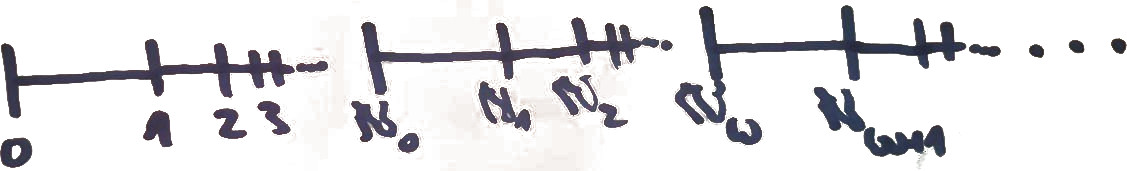
\includegraphics[width=\textwidth]{cardinal-number-line}
  \pause

  \textbf{Def.} The size of the set~$\RR$ of real numbers
  is~\hil{$\boldsymbol{\ccc}$}.
  \medskip

  \textbf{Thm. (Cantor's diagonal argument).} $\ccc > \aleph_0$ (in fact, $\ccc =
  2^{\aleph_0}$).

  \begin{hilblock}
    Where is~$\ccc$ located on the cardinal number line?
  \end{hilblock}
  \vspace*{-0.5em}

  The \hil{continuum hypothesis}~\CH states: ``$\ccc = \aleph_1$.'' Alas:

  \begin{enumerate}\small
    \item \ \\[-1.2em]\mbox{If there is a~\ZFC-proof of~$\neg\CH$, then~\ZFC is
    inconsistent. [Gödel 1938]}
    \item \ \\[-1.2em]\mbox{If there is a~\ZFC-proof of~$\CH$, then~\ZFC is
    inconsistent. [Cohen 1963]}
  \end{enumerate}
  \bigskip

  \centering
  Hence the traditional dream solution:

  \hil{Devise additional axioms to settle~\CH.}
\end{frame}

\begin{frame}{Models of~\ZFC}
  \justifying
  \textbf{Def.} A \hil{model} of~\ZFC is a collection~$M$ together with a
  binary relation on~$M$ for which the axioms of~\ZFC are satisfied.
  \begin{itemize}
    \item Elements of~$M$ are called ``sets of~$M$'', ``what~$M$
    believes to be sets'' or~``$M$-sets''. The relation is written ``$\in$''.
    \item ``$M \models \varphi$'' means: The statement~$\varphi$ holds
    for~$M$-sets.
  \end{itemize}
  \bigskip
  \pause

  \footnotesize
  \textbf{Non-example 1.} Let~$M = \{ \heartsuit \}$ and declare~$\heartsuit
  \in \heartsuit$.

  \textbf{Non-example 2.} Let~$M = \{ \heartsuit \}$ and declare~$\heartsuit
  \not\in \heartsuit$.

  \textbf{Example.} Let~$M$ be the collection of all sets in the platonic
  heaven. Declare~$x \in y$ if and only if~$x$ is actually an
  element of~$y$. \\[0em]
  \bigskip
  \normalsize
  \pause

  \textbf{Rem.} Any model~$M$ of~\ZFC takes a definitive stance on each
  statement: For any mathematical statement~$\varphi$, the
  expression~``$M \models \varphi$'' has a definite truth value.
  \bigskip
  \pause

  \centering
  Embrace the \hil{multiverse}, \\ the entirety of all models of~\ZFC.
\end{frame}

\begin{frame}{Traveling the multiverse}
  \textbf{Def.} (modal operators)
  \begin{enumerate}
    \item \ \\[-1.2em]\mbox{``$\Diamond\varphi$'' means that~$\varphi$ holds in \hil{some}
    extension of the universe.}
    \item \ \\[-1.2em]\mbox{``$\Box\varphi$'' means that~$\varphi$ holds in \hil{every}
    extension of the universe.}
  \end{enumerate}
  \bigskip

  \only<1>{\bigskip\bigskip\centering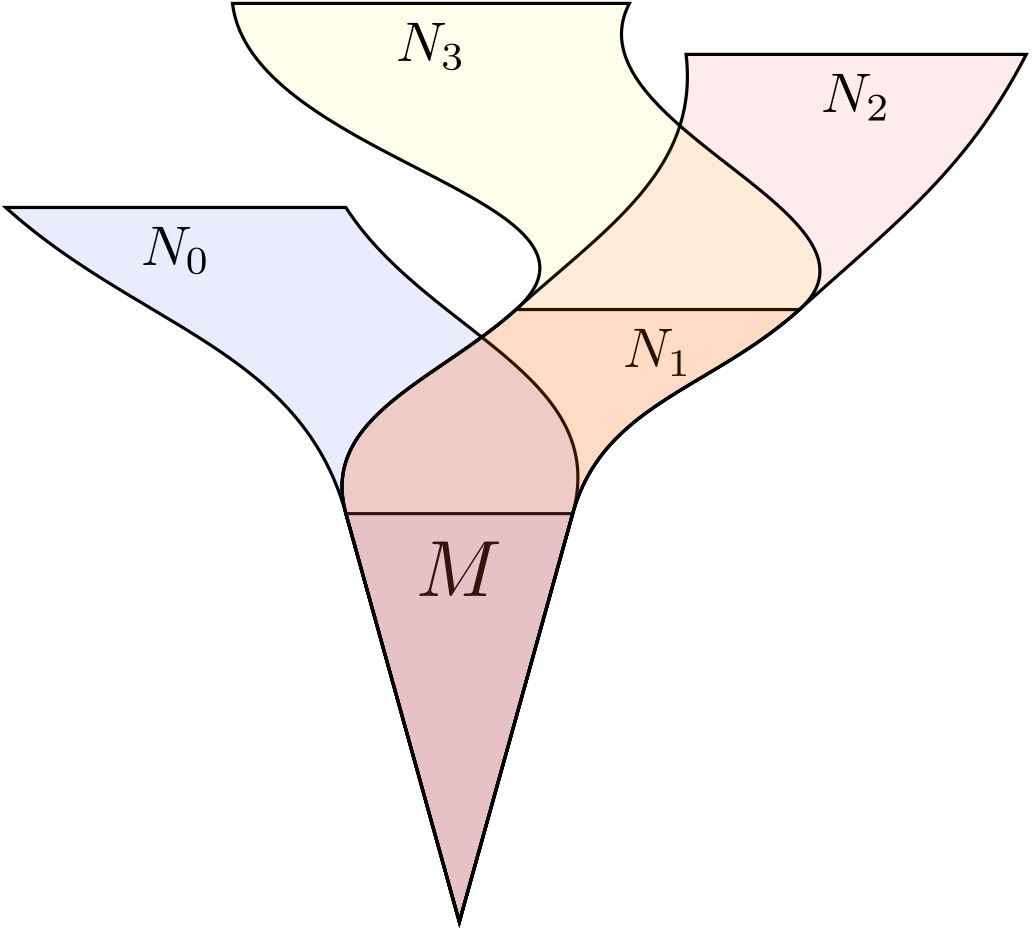
\includegraphics[width=0.4\textwidth]{multiverse}}
  \pause

  \textbf{Def.}
  \begin{enumerate}\justifying
    \item A \hil{switch} is a statement~$\varphi$ such
    that~$\Box((\Diamond\varphi) \wedge (\Diamond(\neg\varphi)))$:

    \small
    No matter where we  travel to from the current universe, there will always
    be a road to a universe in which~$\varphi$ holds and there will always be a
    road to a universe in which~$\varphi$ does not hold.

    \normalsize
    \item A \hil{button} is a statement~$\varphi$ such
    that~$\Box(\Diamond(\Box\varphi))$:

    \small
    No matter where we travel to from the current universe, there will always
    be a road to a universe such that~$\varphi$ holds there and in any further universe
    reachable from there.
  \end{enumerate}
  \bigskip

  \textbf{Example.} \CH is a switch.
\end{frame}

{\usebackgroundtemplate{\begin{minipage}{\paperwidth}\centering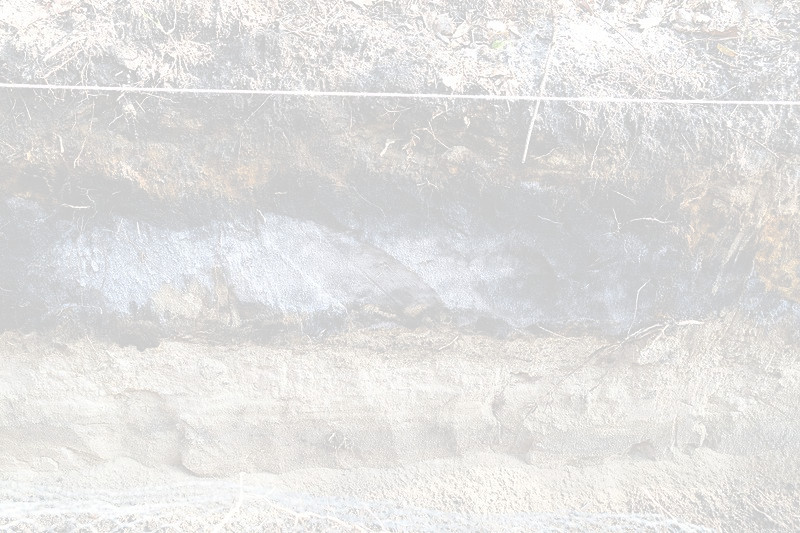
\includegraphics[height=\paperheight]{geology-light}\end{minipage}}
\begin{frame}{Notable features of the multiverse}
  \begin{enumerate}\justifying
    \item The \hil{mirage of uncountability}: Any model is \hil{merely countable}
    from the point of view of a sufficiently larger model.
    \item The \hil{mirage of well-foundedness}: Any model is \hil{ill-founded} from
    the perspective of an appropriate other model.
    \item Some models are maximally rich in that they validate~$(\Diamond(\Box\varphi)) \Rightarrow
    (\Box\varphi)$.
    \item There is a certain Turing machine~$P$ such that for any
    function~$f : \NN \to \NN$, there is some model in
    which~$P$ computes~$f$.
    \item Set-theoretic geology: A \hil{ground} of a model~$M$ is a model~$M'$
    such that~$M$ is an extension of~$M'$. The \hil{mantle} of~$M$ is the
    intersection of all its grounds. \ldots{} an ancient paradise?
  \end{enumerate}
\end{frame}}

\end{document}
